\documentclass[3pt,twocolumn]{elsarticle}
\usepackage[spanish]{babel}
\usepackage[utf8]{inputenc}
\usepackage[T1]{fontenc}
\usepackage{lineno,hyperref}
\modulolinenumbers[5]
\usepackage{graphicx}
\usepackage{subcaption}
\usepackage{listings}
\lstset{language=R, breaklines=true}
\usepackage{amsmath}
\bibliographystyle{elsarticle-num}
\captionsetup[subfigure]{labelformat=brace}

\makeatletter

\renewenvironment{abstract}{\global\setbox\absbox=\vbox\bgroup
  \hsize=\textwidth\def\baselinestretch{1}%
  \noindent\unskip\textbf{Resumen}  % <--- Edit as necessary
 \par\medskip\noindent\unskip\ignorespaces}
 {\egroup}

\def\keyword{%
  \def\sep{\unskip, }%
 \def\MSC{\@ifnextchar[{\@MSC}{\@MSC[2000]}}
  \def\@MSC[##1]{\par\leavevmode\hbox {\it ##1~MSC:\space}}%
  \def\PACS{\par\leavevmode\hbox {\it PACS:\space}}%
  \def\JEL{\par\leavevmode\hbox {\it JEL:\space}}%
  \global\setbox\keybox=\vbox\bgroup\hsize=\textwidth
  \normalsize\normalfont\def\baselinestretch{1}
  \parskip\z@
  \noindent\textit{Palabras clave: }  % <--- Edit as necessary
  \raggedright                         % Keywords are not justified.
  \ignorespaces}

\def\ps@pprintTitle{%
     \let\@oddhead\@empty
     \let\@evenhead\@empty
     \def\@oddfoot{\footnotesize\itshape
       Proyecto final de la unidad de aprendizaje \ifx\@journal\@empty Simulación computacional de nanomateriales  % <--- Edit as necessary
       \else\@journal\fi\hfill\today}%
     \let\@evenfoot\@oddfoot}

\makeatother

\begin{document}

\twocolumn[
\begin{@twocolumnfalse}
\begin{frontmatter}
\title{Modelado de grano grueso de la proteína ubiquitina}
\author{C. A. Estrada}
\address{Facultad de Ingeniería Mecánica y Eléctrica, Universidad Autónoma de Nuevo León}

\begin{abstract}
La ubiquitina es una proteína que regula el reciclaje de otras proteínas dentro de la célula y que tiene relevancia en el ámbito de la nanotecnología, principalmente en el estudio de las interacciones entre proteínas y nanopartículas para estimar sus posibles efectos tóxicos. El conocer la estructura de las proteínas es vital para comprender su función biológica, y la correcta implementación de herramientas bioinformáticas con técnicas de modelado molecular, tales como el modelado de grano grueso (``coarse-grained modeling'', en inglés), permiten la predicción teórica de las estructuras tridimensionales de las proteínas. En el presente trabajo se realizó la simulación con modelado de grano grueso empleando el modelo de campo de fuerza Martini en la dinámica molecular de la ubiquitina humana, para su posterior análisis estructural y de calidad. La ubiquitina modelada por la simulación no alcanzó una calidad satisfactoria, con un RMSD de 0.7 nm, pero obtuvo un patrón de fluctuación RMSF que corresponde con el de la ubiquitina, por lo que las características estructurales del esqueleto de la ubiquitina se conservaron. 
\end{abstract}

\begin{keyword}
Proteína \sep Simulación \sep Ubiquitina \sep GROMACS \sep Martini
\end{keyword}
\end{frontmatter}
\end{@twocolumnfalse}
]

\section{Introducción}
Las proteínas son algunas de las biomoléculas más importantes dentro de la compleja maquinaria que compone a los seres vivos. Un ejemplo de ello es la ubiquitina, una proteína pequeña y de forma globular, compuesta de 76 aminoácidos, cuya función es regular la degradación de otras proteínas de la célula para su reciclaje mediante la unión covalente con el aminoácido lisina de las proteínas blanco, para su posterior degradación intracelular en el proteosoma \cite{BERTICS2014184}. La ubiquitina tiene relevancia en el campo de la nanotecnología aplicada a la medicina, ya que, en el caso de las nanopartículas, al interactuar con los sistemas biológicos las nanopartículas pueden alterar la conformación de las proteínas, conllevando efectos tóxicos \cite{ding2013direct}; con el estudio de la interacción de la ubiquitina con las nanopartículas se pretende comprender los mecanismos con los que las proteínas interactúan con las nanopartículas aplicadas para la liberación de fármacos y conocer mejor los posibles efectos tóxicos de éstas \cite{brancolini2012docking,calzolai2010protein}.

El conocer la estructura de las proteínas es de gran importancia para comprender su función biológica, ya que cada proteína posee una estructura tridimensional específica porque su plegamiento se relaciona directamente con la función que desempeña \cite{de2012}. Para ello, la adecuada adaptación y combinación de herramientas bioinformáticas y técnicas de modelado molecular permiten la predicción teórica de las estructuras tridimensionales de las proteínas \cite{haas2013}. 

La mayoría de las proteínas son demasiado grandes para ser estudiadas con herramientas clásicas de simulación, como el modelado molecular a nivel atómico, por lo que el modelado de grano grueso (``coarse-grained modeling'', en inglés) se convierte en una buena alternativa para ello. En el modelo de grano grueso se reducen los grados de libertad al ignorar algunos de los átomos o mediante la formación de grupos de átomos que son tratados como una sola unidad, en lo que se denomina como ``pseudoátomos'' o granos gruesos \cite{blaszczy}, pero a la vez permite mantener las principales características fisicoquímicas. Los modelos de grano grueso han sido utilizados exitosamente para el estudio de los mecanismos de plegamiento y para la predicción estructural de proteínas \cite{kmiecik}, obteniendo resultados favorables.

En la actualidad, se disponen de diversas aproximaciones de modelado de grano grueso, las cuales varían desde aquellas con una aproximación cuantitativa, como los modelos libres de solventes, hasta aquellos modelos más realistas que incluyen especificidad química \cite{voth2008}. Otra aproximación es la de el campo de fuerza Martini (``Martini force field'', en inglés), el cual es un campo de fuerza empleado en modelado de grano grueso adaptado para simulaciones de dinámica molecular de sistemas biológicos \cite{marrink2007}. El campo de fuerza Martini combina dos estrategias: primero, las interacciones no vinculadas se basan en la reproducción de las energías libres de partición experimentales entre las fases polares y apolares, y, segundo, las interacciones vinculadas se derivan de simulaciones de referencia de todos los átomos. Este modelo emplea un mapeo de cuatro a uno, lo que significa que se promedian cuatro átomos pesados con sus átomos de hidrógeno asociados y se representan como un solo centro de interacción o pseudoátomo; además, solo se definen cuatro tipos de sitios de interacción: polares, apolares, no polares y con carga, y, a su vez, a cada partícula se le asigna cierto número de subtipos de estas cuatro interacciones, lo que permite representar de manera más precisa la naturaleza química de la molécula \cite{marrink2007}. El modelo Martini ha sido adaptado para su empleo en proteínas \cite{monticelli2008}, en donde cada residuo (es decir, cada aminoácido que forma parte de la cadena polipeptídica) posee un pseudoátomo en el esqueleto de la proteína y desde cero a cuatro pseudoátomos de las cadenas laterales, dependiendo del tipo de residuo. 

En el presente trabajo se realizó una simulación con modelado de grano grueso de la ubiquitina humana empleando el modelo de campo de fuerza Martini, para su posterior análisis estructural y de calidad, los cuales se describen en mayor detalle en la sección de resultados y discusión.

\section{Experimentación}
\subsection{Herramientas}
La simulación se realizó en una laptop HP Pavilion con un procesador AMD Ryzen 3. Para la simulación de la proteína se utilizó el paquete de software de libre uso GROMACS 2020.1 \cite{gromacs}, así como el software Python 2.7 \cite{python}. La visualización de las estructuras de las proteínas se realizó con el software de libre uso Jmol \cite{jmol}, y el análisis de resultados con el paquete estadístico R versión 4.0.2 \cite{R}.
\subsection{Simulación}
La simulación se llevó a cabo utilizando el archivo proveniente de Protein Data Bank para la ubiquitina humana con el código de indentificación 1UBQ \cite{proteina}, el cual contiene la estructura atomística de la proteína requerida para la simulación, y cuyas características generales se presentan en el cuadro \ref{pdb}. Utilizando el código de uso libre para el modelado de grano grueso con el campo de fuerza Martini \cite{martinize}, se convirtió la estructura atomística de la ubiquitina en una estructura de grano grueso en Python 2.7, especificando la generación de la lista de los átomos involucrados, así como la determinación de la clasificación de la estructura secundaria del esqueleto de la proteína. Posteriormente, utilizando la estructura de grano grueso de la ubiquitina en GROMACS se especificó las condiciones límite periódicas (características de la caja en que se produce la simulación) utilizando una caja de forma dodecaédrica (óptima para las proteínas de conformación globular) con una distancia mínima de 1 nm entre la proteína y cualquier borde de la caja, y se procedió a realizar una minimización en vacío de 100 pasos. Después, se realizó la solvatación del sistema utilizando una caja de agua cuyo sistema está equilibrado (temperatura de 300 K, 1 bar de presión y 2,000 pseudoátomos de agua) y se procedió a una minimización de energía de 100 pasos, con la subsecuente equilibración del sistema con una duración de 10,000 pasos. A partir de ello se realizó la simulación de dinámica molecular del sistema completo con una duración de 3,000,000 pasos. Una vez finalizada la simulación, se convirtió a las trayectorias generadas de tal manera que la traslación y rotación de la ubiquitina sean removidas, y con ello realizar los análisis estándar que se describen en la siguiente sección.  

\begin{table}[h]
\begin{center}
\caption{Contenido de la macromolécula 1UBQ.}
\label{pdb}
\begin{tabular}{r r}
\hline
Peso total de la estructura&8.58 kDa\\
Cantidad de átomos&660\\
Cantidad de residuos&76\\
Cadenas de proteína únicas&1\\
\hline
\end{tabular}
\end{center}
\end{table}
\subsection{Análisis de resultados}
Utilizando GROMACS se calcula la desviación cuadrática media de las posiciones atómicas (RMSD, por sus siglas en inglés) y la fluctuación cuadrática media (RMSF, por sus siglas en inglés), mientras que los datos generados son graficados utilizando el paquete estadístico R. La visualización de la nueva estructura de la ubiquitina generada, así como la estructura original, se realizó utilizando Jmol.

\section{Resultados y discusión}
En la figura \ref{estructura} se presentan las estructuras tridimensionales en un modelo de bolas y varillas generados en Jmol de la ubiquitina original proveniente de Protein Data Bank, la misma estructura después de haber sido convertida a granos gruesos (pseudoátomos) y la proteína generada al finalizar la simulación. El código de colores indica los aminoácidos de acuerdo con sus propiedades, por lo que se puede ubicar a simple vista la localización aproximada de los residuos que componen tanto a la proteína original como a la proteína generada por la simulación; se observa que la ubiquitina original posee una gran cantidad de esferas, ya que se modeló su estructura atomística, mientras que la estructura convertida a granos gruesos posee menor cantidad, lo que indica que la conversión fue exitosa. La proteína generada por la simulación posee los granos gruesos de la conversión con sus respectivas interacciones, representando de manera simplista la estructura tridimensional original de la ubiquitina, en donde se observa que la posición aproximada de las regiones de cada aminoácido se conservó después de la simulación.

\begin{figure*}
\begin{subfigure}{0.49\textwidth}
\centering
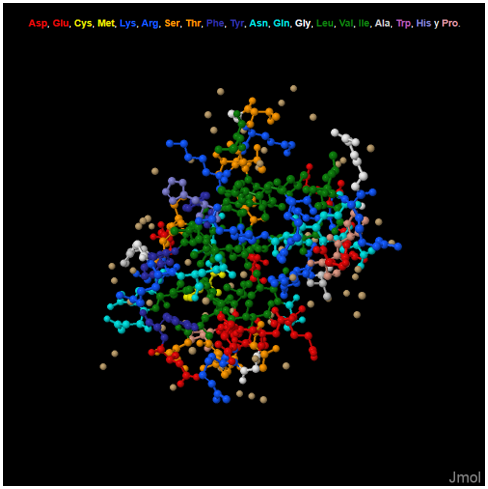
\includegraphics[height=7cm,width=\linewidth]{pPDB.png}
\caption{Ubiquitina original.}
\label{1}
\end{subfigure}\hfill
\begin{subfigure}{0.49\textwidth}
\centering
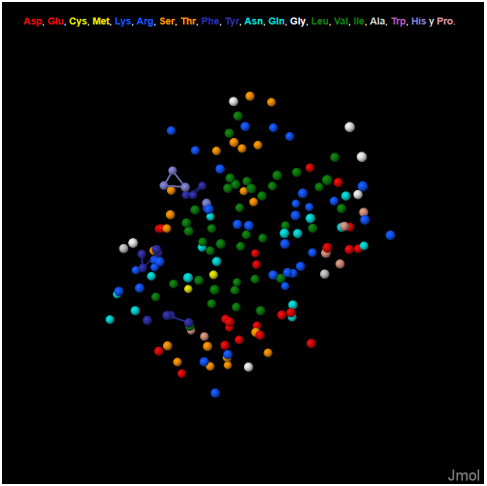
\includegraphics[height=7cm,width=\linewidth]{pCG.png}
\caption{Ubiquitina convertida a granos gruesos.}
\label{2}
\end{subfigure}\hfill
\begin{subfigure}{0.49\textwidth}
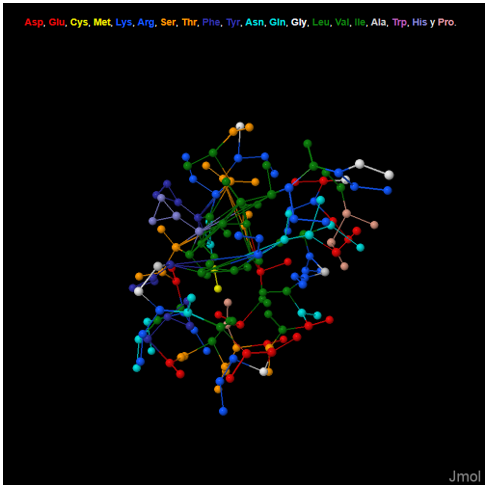
\includegraphics[height=7cm,width=\linewidth]{pMD.png}
\caption{Ubiquitina simulada.}
\label{3}
\end{subfigure}\hfill
\caption{Estructuras tridimensionales de la ubiquitina en modelo de bolas y varillas generadas con Jmol.}
\label{estructura}
\end{figure*}

En la figura \ref{rmsf} se presenta la desviación promedio de cada residuo que compone a la proteína simulada a través del tiempo (RMSF); esta medida es un indicador de las porciones de la estructura que fluctúan más a partir de su estructura promedio \cite{fluctuacion}, lo que representa a las regiones flexibles de la proteína, que en este caso serían los bucles. Los bucles se encuentran en particular en las superficies de proteínas globulares \cite{loops}, como la ubiquitina, lo que explica que se haya presentado un RMSF alto en muchos de los residuos; además, este patrón coincide con el reportado previamente para la ubiquitina \cite{simuubq}, ya que los patrones de fluctuación del esqueleto de las proteínas tienden a conservarse \cite{conserva}, mientras que las leves variaciones se deben a la dinámica molecular en particular de la simulación.

\begin{figure}[ptb]
\begin{center}
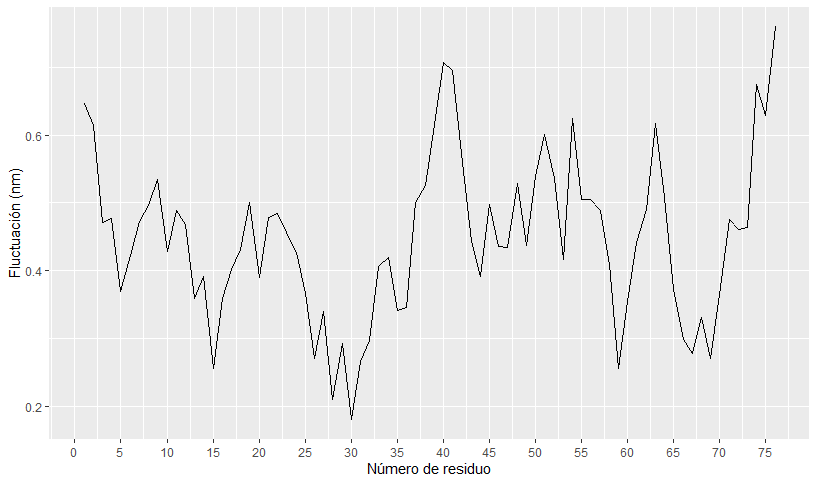
\includegraphics[width=\linewidth]{rmsf.png}
\end{center}
\caption{Fluctuación cuadrática media (RMSF) en función de cada número de residuo de la secuencia a través del tiempo de la ubiquitina simulada.\label{rmsf}}
\end{figure}

Finalmente, en la figura \ref{rmsd} se presenta la desviación cuadrática media de las posiciones atómicas (RMSD) a partir de la estructura cristalográfica a través del tiempo, la cual es una medida acerca de la exactitud del modelo predicho. Para la ubiquitina simulada, se observa que el RMSD aumenta su valor a través del tiempo hacia una especie de meseta, lo que indica que la estructura tiende a buscar estabilidad a lo largo del tiempo con respecto a la estructura de referencia, pero al tratarse de valores que llegan hasta aproximadamente 0.7 nm, la conformación de la proteína no es estable. El valor de RMSD al finalizar la simulación es de aproximadamente 0.7 nm, el cual se encuentra muy por encima del valor RMSD reportado como control de calidad para simulaciones de proteínas, que es de menos de 0.2 nm \cite{spoel}; esto pudo deberse a que la simulación, por simplicidad, se realizó utilizando una caja de agua pura, evitando la adición de iones, y es un hecho que las proteínas requieren de cierta cantidad de iones para mantener su estabilidad \cite{sales}. En otros reportes con los mismos parámetros utilizados en este trabajo, el RMSD de la ubiquitina mantuvo valores por debajo de los 0.2 nm, con la diferencia que se tomó en cuenta la adición de algunos iones \cite{simuubq}, lo que corrobora que fue la omisión de este parámetro lo que causó los valores tan altos obtenidos.

\begin{figure}[ptb]
\begin{center}
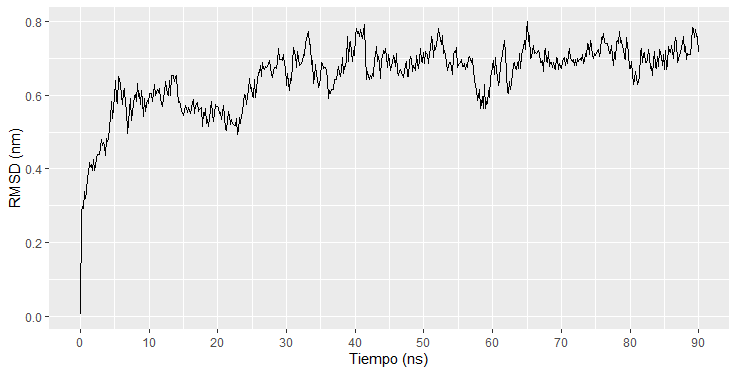
\includegraphics[width=\linewidth]{rmsd.png}
\end{center}
\caption{Desviación cuadrática media de las posiciones atómicas (RMSD) a partir de la estructura cristalográfica en función del tiempo.\label{rmsd}}
\end{figure}


\section{Conclusiones}
La ubiquitina modelada por grano grueso obtuvo una estructura tridimensional similar a la ubiquitina original, lo cual se ve corroborado por el RMSF obtenido, que coincide con el patrón de fluctuación del esqueleto de la ubiquitina reportado en la literatura. No obstante, el modelo producido obtuvo un RMSD de aproximadamente 0.7 nm al finalizar la simulación, por lo que no alcanzó una calidad satisfactoria, ya que esto indica que su conformación es inestable.

Se requeriría realizar la simulación nuevamente en el futuro, incluyendo iones en la fase de solvatación del sistema para incrementar la estabilidad de la ubiquitina a lo largo del tiempo. De igual forma, se podrían incorporar nuevos parámetros que permitan el estudio de su interacción con otras proteínas, o incluso nanopartículas.

\section{Agradecimientos}
Se agradece encarecidamente al Lic. Juan Garza por su asesoría para la instalación de GROMACS, al igual que a la Dra. Elisa Schaeffer por sus correcciones en la estructura original del trabajo.

\bibliography{referencias}

\end{document}

